\chapter{Atbulinis išvedimas}

\section{Užduotis}

Parašyti programą, kuri, kaip pradinius duomenis gavusi trejetą
$<R, F, G>$, panaudodama atbulinio išvedimo sistemą nustatytų
ar tikslas $G$ yra išvedamas ir jei taip, tai kokias produkcijas
turime pritaikyti, kad jį gautume.

\section{Pseudo kodas}

\label{sec:bc:pseudo}

Pradiniai duomenys:
\begin{description}
  \item[$R$] – taisyklių sąrašas;
  \item[$F$] – pradinių faktų aibė;
  \item[$G$] – ieškomas tikslas.
\end{description}

Rezultatas:
\begin{description}
  \item[$Q$] – panaudotų taisyklių seka arba „nesėkmė“.
\end{description}

Kiti kintamieji:
\begin{description}
  \item[$K$] – panaudotų taisyklių sekos dalis;
  \item[$N$] – „naujų“ faktų aibė;
  \item[$P$] – ieškomų tikslų aibė.
\end{description}

\begin{algorithmic}[1]
  \Function{atbulinis išvedimas}{$R, F, G, P := \left\{ G \right\}$}
    \If{$G \in F \lor G \in N$} \label{bc:pseudo:goal_in_facts}
      \State \Return $\emptyset$ \label{bc:pseudo:emptyset}
    \Else
      \ForAll{$r \in R \land r$ išvada yra $G \land$ nė viena iš $r$
              prielaidų $\not\in P$} \label{bc:pseudo:rule_iter}
        \State $Q := \left( \right)$ \label{bc:pseudo:initial_Q}
        \ForAll{$g \in r$ prielaidos} \label{bc:pseudo:premise_iter}
          \State $K := $ atbulinis išvedimas$(%
            R\setminus \left\{ r \right\}, F, g,%
            P \cup \left\{ g \right\})$; \label{bc:pseudo:recursion}
          \If{$K =$ nesėkmė} \label{bc:pseudo:rule:fail}
            \State $Q :=$ nesėkmė;
            \State break
          \Else \label{bc:pseudo:rule:success}
            \State $Q := Q \cup K$;
          \EndIf
          \If{$Q \neq$ nesėkmė} \label{bc:pseudo:success}
            \State Pridedame $G$ į $N$. \label{bc:pseudo:add_fact}
            \State \Return $Q \cup \left\{ R \right\}$;%
              \label{bc:pseudo:return_succ}
          \EndIf
        \EndFor
      \EndFor
      \State \Return nesėkmė; \label{bc:pseudo:failure}
    \EndIf
  \EndFunction
\end{algorithmic}

\section{Realizacija}

Atbulinio išvedimo algoritmo, pateikto \ref{sec:bc:pseudo}
skyrelyje, realizacija:

\pythonai{source}{backwardchaining.BackwardChaining.recursion}

\section{Pavyzdžiai}

\subsection{Pirmasis pavyzdys: paprastas atvejis}

\begin{pythonaienv}[bc]
# Vytauto Astrausko failas.
1. Taisyklės.
ZFB                                     # R1: F, B → Z
FCD                                     # R2: C, D → F
DA                                      # R3: A → D

2. Faktai.
ACB

3. Tikslas.
Z
\end{pythonaienv}

\subsection{Antrasis pavyzdys: du išvedimo keliai}

\begin{pythonaienv}[bc]
# Vytauto Astrausko failas.
1. Taisyklės.
ZD                                      # R1: D → Z
DC                                      # R2: C → D
CB                                      # R3: B → C
GA                                      # R4: A → G
ZG                                      # R5: G → Z
BA                                      # R6: A → B

2. Faktai.
A

3. Tikslas.
Z
\end{pythonaienv}

\subsection{Trečiasis pavyzdys: du išvedimo keliai (taisyklės kita tvarka)}

\begin{pythonaienv}[bc]
# Vytauto Astrausko failas.
1. Taisyklės.
GA                                      # R1: A → G
ZD                                      # R2: D → Z
DC                                      # R3: C → D
CB                                      # R4: B → C
BA                                      # R5: A → B
ZG                                      # R6: G → Z

2. Faktai.
A

3. Tikslas.
Z
\end{pythonaienv}

\subsection{Ketvirtasis pavyzdys: klaidinančios taisyklės}

\begin{pythonaienv}[bc]
# Vytauto Astrausko failas.
1. Taisyklės.
ZZ                                      # R1: Z → Z
ZVA                                     # R2: V, A → Z
ZVAZ                                    # R3: V, A, Z → Z
ZABCDEFGHIJKLMNOPRST                    # R4: A, B, C, D, E, F, G, H, I, J, K, L, M, N, O, P, R, S, T → Z
ZFB                                     # R5: F, B → Z
FCD                                     # R6: C, D → F
DA                                      # R7: A → D
LA                                      # R8: A → L
KL                                      # R9: L → K
AB                                      # R10: B → A
MD                                      # R11: D → M

2. Faktai.
ACB

3. Tikslas.
Z
\end{pythonaienv}

\subsection{Penktasis pavyzdys: ilgas antecedentas}

\begin{pythonaienv}[bc]
# Vytauto Astrausko failas.
1. Taisyklės.
ZG                                      # R1: G → Z
GA                                      # R2: A → G
BA                                      # R3: A → B
CB                                      # R4: B → C
DC                                      # R5: C → D
ZD                                      # R6: D → Z
HABGCDZ                                 # R7: A, B, G, C, D, Z → H

2. Faktai.
A

3. Tikslas.
H
\end{pythonaienv}

\subsection{Šeštasis pavyzdys: išvedimas neegzistuoja}

\begin{pythonaienv}[bc]
# Vytauto Astrausko failas.
1. Taisyklės.
FCD                                     # R1: C, D → F
DA                                      # R2: A → D
LA                                      # R3: A → L
KL                                      # R4: L → K
AB                                      # R5: B → A
MD                                      # R6: D → M
ZFB                                     # R7: F, B → Z

2. Faktai.
ACB

3. Tikslas.
H
\end{pythonaienv}

\subsection{Septintasis pavyzdys: tikslas tarp prielaidų}

\begin{pythonaienv}[bc]
# Vytauto Astrausko failas.
1. Taisyklės.
FCD                                     # R1: C, D → F
DA                                      # R2: A → D
LA                                      # R3: A → L
KL                                      # R4: L → K
AB                                      # R5: B → A
MD                                      # R6: D → M
ZFB                                     # R7: F, B → Z

2. Faktai.
ACB

3. Tikslas.
B
\end{pythonaienv}

\subsection{Aštuntasis pavyzdys: devynių produkcijų DC}

\begin{pythonaienv}[bc]
# Vytauto Astrausko failas.
1. Taisyklės.
ZDC                                     # R1: D, C → Z
DC                                      # R2: C → D
CB                                      # R3: B → C
BA                                      # R4: A → B
AD                                      # R5: D → A
DT                                      # R6: T → D
AG                                      # R7: G → A
BH                                      # R8: H → B
CJ                                      # R9: J → C

2. Faktai.
T

3. Tikslas.
Z
\end{pythonaienv}

\subsection{Devintasis pavyzdys: devynių produkcijų CD}

\begin{pythonaienv}[bc]
# Vytauto Astrausko failas.
1. Taisyklės.
ZCD                                     # R1: C, D → Z
DC                                      # R2: C → D
CB                                      # R3: B → C
BA                                      # R4: A → B
AD                                      # R5: D → A
DT                                      # R6: T → D
AG                                      # R7: G → A
BH                                      # R8: H → B
CJ                                      # R9: J → C

2. Faktai.
T

3. Tikslas.
Z
\end{pythonaienv}

\subsection{Dešimtasis pavyzdys: labirintas}

\subsubsection{Labirinto žemėlapis}

\begin{figure}[H]
  \centering
  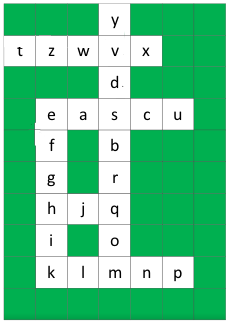
\includegraphics[]{content/map.png}
  \caption{Labirinto žemėlapis}
  \label{fig:bc:map}
\end{figure}

\begin{pythonaienv}[bc]
# Vytauto Astrausko failas.
1. Taisyklės.
Ft                                      # R1: t → F
Fy                                      # R2: y → F
ds                                      # R3: s → d
sd                                      # R4: d → s
as                                      # R5: s → a
sa                                      # R6: a → s
bs                                      # R7: s → b
sb                                      # R8: b → s
cs                                      # R9: s → c
sc                                      # R10: c → s
vd                                      # R11: d → v
dv                                      # R12: v → d
yv                                      # R13: v → y
vy                                      # R14: y → v
wv                                      # R15: v → w
vw                                      # R16: w → v
xv                                      # R17: v → x
vx                                      # R18: x → v
wz                                      # R19: z → w
zw                                      # R20: w → z
tz                                      # R21: z → t
zt                                      # R22: t → z
ea                                      # R23: a → e
ae                                      # R24: e → a
fe                                      # R25: e → f
ef                                      # R26: f → e
gf                                      # R27: f → g
fg                                      # R28: g → f
hg                                      # R29: g → h
gh                                      # R30: h → g
ih                                      # R31: h → i
hi                                      # R32: i → h
jh                                      # R33: h → j
hj                                      # R34: j → h
ki                                      # R35: i → k
ik                                      # R36: k → i
lk                                      # R37: k → l
kl                                      # R38: l → k
ml                                      # R39: l → m
lm                                      # R40: m → l
om                                      # R41: m → o
mo                                      # R42: o → m
nm                                      # R43: m → n
mn                                      # R44: n → m
qo                                      # R45: o → q
oq                                      # R46: q → o
rq                                      # R47: q → r
qr                                      # R48: r → q
jq                                      # R49: q → j
qj                                      # R50: j → q
br                                      # R51: r → b
rb                                      # R52: b → r
pn                                      # R53: n → p
np                                      # R54: p → n
uc                                      # R55: c → u
cu                                      # R56: u → c

2. Faktai.
s

3. Tikslas.
F
\end{pythonaienv}

\subsubsection{Labirintą atitinkantis grafas su sprendimu}

\begin{pythonaienv}[graph|graph:228|Grafas.]
digraph G { // graph-invoke-bc-solve-2: 28 
node [fixedsize="true", fontsize=8, width="0.2cm", height="0.2cm"];
edge [arrowsize="1.5", fontsize=8];
node [shape="box"]; s; 
node [shape="box"]; t; 
edge [arrowsize="1.5", label="R1"]; t -> F; 
node [shape="box"]; y; 
edge [arrowsize="0.7", label="R2"]; y -> F; 
edge [arrowsize="1.5", label="R3"]; s -> d; 
node [shape="box"]; d; 
edge [arrowsize="0.7", label="R4"]; d -> s; 
edge [arrowsize="0.7", label="R5"]; s -> a; 
node [shape="box"]; a; 
edge [arrowsize="0.7", label="R6"]; a -> s; 
edge [arrowsize="0.7", label="R7"]; s -> b; 
node [shape="box"]; b; 
edge [arrowsize="0.7", label="R8"]; b -> s; 
edge [arrowsize="0.7", label="R9"]; s -> c; 
node [shape="box"]; c; 
edge [arrowsize="0.7", label="R10"]; c -> s; 
edge [arrowsize="1.5", label="R11"]; d -> v; 
node [shape="box"]; v; 
edge [arrowsize="0.7", label="R12"]; v -> d; 
edge [arrowsize="0.7", label="R13"]; v -> y; 
edge [arrowsize="0.7", label="R14"]; y -> v; 
edge [arrowsize="1.5", label="R15"]; v -> w; 
node [shape="box"]; w; 
edge [arrowsize="0.7", label="R16"]; w -> v; 
edge [arrowsize="0.7", label="R17"]; v -> x; 
node [shape="box"]; x; 
edge [arrowsize="0.7", label="R18"]; x -> v; 
node [shape="box"]; z; 
edge [arrowsize="0.7", label="R19"]; z -> w; 
edge [arrowsize="1.5", label="R20"]; w -> z; 
edge [arrowsize="1.5", label="R21"]; z -> t; 
edge [arrowsize="0.7", label="R22"]; t -> z; 
edge [arrowsize="0.7", label="R23"]; a -> e; 
node [shape="box"]; e; 
edge [arrowsize="0.7", label="R24"]; e -> a; 
edge [arrowsize="0.7", label="R25"]; e -> f; 
node [shape="box"]; f; 
edge [arrowsize="0.7", label="R26"]; f -> e; 
edge [arrowsize="0.7", label="R27"]; f -> g; 
node [shape="box"]; g; 
edge [arrowsize="0.7", label="R28"]; g -> f; 
edge [arrowsize="0.7", label="R29"]; g -> h; 
node [shape="box"]; h; 
edge [arrowsize="0.7", label="R30"]; h -> g; 
edge [arrowsize="0.7", label="R31"]; h -> i; 
node [shape="box"]; i; 
edge [arrowsize="0.7", label="R32"]; i -> h; 
edge [arrowsize="0.7", label="R33"]; h -> j; 
node [shape="box"]; j; 
edge [arrowsize="0.7", label="R34"]; j -> h; 
edge [arrowsize="0.7", label="R35"]; i -> k; 
node [shape="box"]; k; 
edge [arrowsize="0.7", label="R36"]; k -> i; 
edge [arrowsize="0.7", label="R37"]; k -> l; 
node [shape="box"]; l; 
edge [arrowsize="0.7", label="R38"]; l -> k; 
edge [arrowsize="0.7", label="R39"]; l -> m; 
node [shape="box"]; m; 
edge [arrowsize="0.7", label="R40"]; m -> l; 
edge [arrowsize="0.7", label="R41"]; m -> o; 
node [shape="box"]; o; 
edge [arrowsize="0.7", label="R42"]; o -> m; 
edge [arrowsize="0.7", label="R43"]; m -> n; 
node [shape="box"]; n; 
edge [arrowsize="0.7", label="R44"]; n -> m; 
edge [arrowsize="0.7", label="R45"]; o -> q; 
node [shape="box"]; q; 
edge [arrowsize="0.7", label="R46"]; q -> o; 
edge [arrowsize="0.7", label="R47"]; q -> r; 
node [shape="box"]; r; 
edge [arrowsize="0.7", label="R48"]; r -> q; 
edge [arrowsize="0.7", label="R49"]; q -> j; 
edge [arrowsize="0.7", label="R50"]; j -> q; 
edge [arrowsize="0.7", label="R51"]; r -> b; 
edge [arrowsize="0.7", label="R52"]; b -> r; 
edge [arrowsize="0.7", label="R53"]; n -> p; 
node [shape="box"]; p; 
edge [arrowsize="0.7", label="R54"]; p -> n; 
edge [arrowsize="0.7", label="R55"]; c -> u; 
node [shape="box"]; u; 
edge [arrowsize="0.7", label="R56"]; u -> c; 
}

\end{pythonaienv}
